\chapter{Actor-Critic Algorithms}
Recall from last chapter, we derived the policy gradient theorem:
$$\nabla_\theta J(\theta) \simeq \frac{1}{N}\sum_{i=1}^N\left(\sum_{t=1}^T\nabla_\theta \log\pi_\theta(a_{i,t}|s_{i,t})\right)\left(\sum_{t'=1}^T r(s_{i,t'},a_{i,t'})\right)$$
where we defined the summed reward as the ``reward-to-go'' function $\hat{Q}_{i,t}$, and it represents the estimate of expected reward if we take action $a_{i,t}$ in state $s_{i,t}$. We have shown that this estimate has very high variance, and we shall see how we can improve policy gradients from using better estimation of the reward-to-go function.

\section{Reward-to-Go}
Let us take a closer look at the reward-to-go. To improve the estimation, one way is to get closer to the precise value of the reward-to-go. We can define the reward-to-go using expectation:
$$Q(s_t,a_t) = \sum_{t'=t}^T \mathbb{E}_{\pi_\theta}\left[r(s_{t'},a_{t'})|s_t,a_t\right]$$
this is the \textbf{true, expected} value of the reward-to-go.

Therefore, one could imagine using this true expected value, combined with our original Monte Carlo approximation to yield a better estimate:
$$\nabla_\theta J(\theta) \simeq \frac{1}{N}\sum_{i=1}^N\sum_{t=1}^T\nabla_{\theta}\log \pi_\theta (a_{i,t}|s_{i,t})Q(s_{i,t},a_{i,t})$$.

\section{Using Baselines}
As we have seen in last chapter, one can reduce the high variance of the policy gradient using baselines. We have also seen that it is possible to calculate the optimal baseline value to yield the minimum variance, although people often use the average reward for sake of simplicity.

Motivated by this, let us recall the definition of the value function (defined in the introduction section):
$$V(s_t) = \mathbb{E}_{a_t\sim \pi_\theta(a_t|s_t)}\left[Q(s_t,a_t)\right]$$
By definition, the value function is the average of Q-function value.

Similarly, we can use the \textbf{average} reward-to-go as a baseline to reduce the variance. Specifically, we could use the value function $V(s_t)$ as the baseline, thus improving the estimate of the gradient in the following way:
$$\nabla_\theta J(\theta) \simeq \frac{1}{N}\sum_{i=1}^N\sum_{t=1}^T\nabla_{\theta}\log \pi_\theta (a_{i,t}|s_{i,t})\left(Q(s_{i,t},a_{i,t}) - V(s_{i,t})\right)$$
and the value function we used is a better approximation of the baseline $b_t = \frac{1}{N}\sum_i Q(s_{i,t},a_{i,t})$.

What have we done here? What is the intuition behind subtracting the value function from the Q-function? Essentially, we are quantifying how much an action $a_{i,t}$ is better than the average actions. In some sense, it measures the \textbf{advantage} of applying an action over the average action. Therefore, to formalize our intuition, let us define the advantage as follows:
$$A^\pi(s_t,a_t) = Q^\pi(s_t,a_t) - V^\pi(s_t)$$
which quantitatively measures how much better action $a_t$ is.

Putting it all together, now a better baseline-backed policy gradient estimate using Monte Carlo estimate can be written as:
$$\nabla_\theta J(\theta) \simeq \frac{1}{N}\sum_{i=1}^N\sum_{t=1}^T\nabla_{\theta}\log \pi_\theta (a_{i,t}|s_{i,t})A^\pi(s_{i,t},a_{i,t})$$.

\section{Value Function Fitting}
The better the estimate of the advantage function, the lower the variance, and we can have better policy gradient. Let us massage the definition of the Q-function a little in order to find some interesting mathematical relations between $Q$ and $V$:
\begin{align*}
    Q^\pi(s_t,a_t) &= \sum_{t'=t}^T \mathbb{E}_{\pi_\theta}\left[r(s_{t'},a_{t'})|s_t,a_t\right]\\
    &= r(s_t,a_t)+\sum_{t'=t+1}^T \mathbb{E}_{\pi_\theta}\left[r(s_{t'},a_{t'})|s_t,a_t\right]\\
    &= r(s_t,a_t) + V^\pi(s_{t+1})\\
    &= r(s_t,a_t) + \mathbb{E}_{s_{t+1}\sim p(s_{t+1}|s_t,a_t)}\left[V^\pi(s_{t+1})\right]
\end{align*}
The last expectation of the value function is used because we do not know what the next state actually is. Note that we can be a little crude with respect to that expectation in such a way that we just use the full value function $V^\pi(\cdot)$ on one single sample of the next state, and use the value as the expectation, ignoring the fact that there are multiple other next states. With this estimate, we can plug into the advantage function:
$$A^\pi(s_t,a_t) \simeq r(s_t,a_t) + V^\pi(s_{t+1}) - V^\pi(s_t)$$

Therefore, it is almost enough to just approximate the value function, which solely depends on state, to generate approximations of other functions. To achieve this, we can use a neural network to fit our value function $V(s)$, and use the fit value function to approximate our policy gradient, as illustrated in Fig. \ref{fig:fitV} 
\begin{figure}
    \centering
    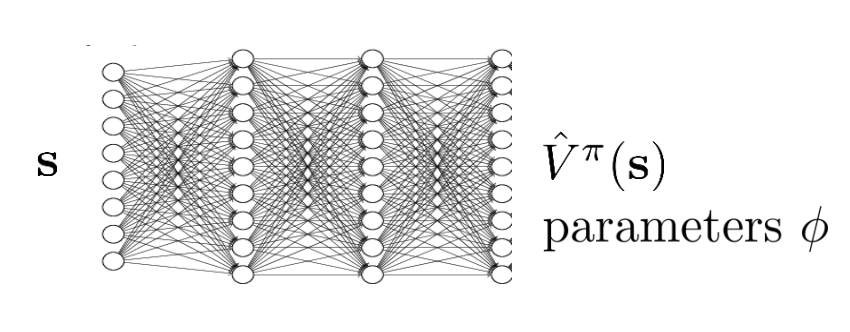
\includegraphics[scale=0.5]{figures/fitV.png}
    \caption{Fitting the value function}
    \label{fig:fitV}
\end{figure}

\section{Policy Evaluation}
Here in this section, we discuss the process and purpose of fitting the value function.

\subsection{Why Do We Evaluate a Policy}
Policy evaluation is a process that given a fixed policy $\pi$, we figure out how good it is by fitting the value function $V^\pi(\cdot)$ by using this expectation:
$$V^\pi(s_t) = \sum_{t'=t}^T\mathbb{E}_{\pi_\theta}\left[r(s_{t'},a_{t'})|s_t\right]$$
Having the value function allows us to figure out how good the policy is because the reinforcement learning objective can be equivalently written as $J(\theta) = \mathbb{E}_{s_1\sim p(s_1)}\left[V^\pi(s_1)\right]$, where we take the expectation of the value function value of the initial state over all possible initial states.
\subsection{How to Evaluate a Policy}
To evaluate a policy, we can use an approach similar to the policy gradient - Monte Carlo approximation. Specifically, we can estimate the value function by summing up the reward collected from time step $t$:
$$V^\pi(s_t) \simeq \sum_{t'=t}^T r(s_{t'},a_{t'})$$
and if we are able to reset the simulator, we could indeed ameliorate this estimate by taking multiple samples ($N$) as follows:
$$V^\pi(s_t) \simeq \frac{1}{N}\sum_{i=1}^N\sum_{t'=t}^T r(s_{i,t'},a_{i,t'})$$
In practice, we can just use the single sample approximation.

Here is a question, if our original objective is to use $V^\pi$ to reduce the variance, but we end up using a single sample estimation to estimate $V^\pi$, does it actually help? The answer is yes, because we are using a neural net to fit the Monte Carlo targets from a variety of different states, so even though we do single sample estimate, the value function does generalize when we visit similar states. 

\subsection{Monte Carlo Evaluation with Function Approximation}
To fit our value function, we could use a supervised learning approach. Essentially, we can use our single sample estimation of the value function as our function value, and fit a function that maps the states to the value function values. Therefore, our training data will be $\left\{(s_{i,t}, \sum_{t'=t}^Tr(s_{i,t'},a_{i,t'}))\right\}$, and we denote the function value labels as $y_{i,t}$, and we define a typical supervised regression loss function which we try to minimize as $\mathcal{L}(\phi) = \frac{1}{2}\sum_i\lvert|\hat{V}_\phi^\pi(s_i)-y_i|\rvert^2$. 

\subsection{Improving the Estimate Using Bootstrap}
In fact, we can improve our training process because the original applied target $y_{i,t}$ is not perfect. We could use a technique called bootstrapping. Recall the definition of our ideal target in the supervised regression:
$$\begin{aligned}
    y_{i,t} &= \sum_{t'=t}^T\mathbb{E}_{\pi_\theta}\left[r(s_{t'},a_{t'})|s_{i,t}\right]\\
    & \simeq r(s_{i,t},a_{i,t})+\sum_{t'=t+1}^T\left[r(s_{t'},a_{t'})|s_{i,t+1}\right]\\
    & \simeq  r(s_{i,t},a_{i,t}) + V^\pi(s_{i,t+1})
\end{aligned}$$
, compared with our Monte Carlo targets: $y_{i,t} = \sum_{t'=t}^T r(s_{i,t'},a_{i,t'})$.

Bootstrapping means applying our previous estimation on our current estimation. In our ideal targets, the last estimation is accurate if we knew the actual $V^\pi$. But if the actual is not known, we can just apply bootstrapping by using the current fit estimate $\hat{V}^\pi_\phi$ to estimate the next state's value: $\hat{V}^\pi_\phi(s_{i,t+1})$. Such an estimate is biased, but it has low variance.

Consequently, our training data using bootstrapping becomes: $\left\{(s_{i,t}, r(s_{i,t},a_{i,t}) +\hat{V}^\pi_\phi(s_{i,t+1})) \right\}$. Such bootstrapped targets work well with highly stochastic environments. 

\section{Batch Actor-Critic Algorithm}
Now we are ready to devise our first actor-critic algorithm. The reason why we call it actor-critic is that we use a critic (value function) to decrease the high variance of the actor (Q-function). The full algorithm is shown in Alg. \ref{alg:batchac} and we call it a batch algorithm because it is not online. We shall see the online version later.
\begin{algorithm}[t!]
\caption{Batch Actor-Critic Algorithm}
\begin{algorithmic}[1]
\label{alg:batchac}
\REQUIRE Base policy $\pi_\theta(a_t|s_t)$

\WHILE{true}
    \STATE Sample $\{s_i,a_i\}$ from $\pi_\theta(a|s)$ (run it on a robot)
    \STATE Fit $\hat{V}_\phi(s)$ to sampled reward sums
    \STATE Evaluate $\hat{A}^\pi(s_i,a_i) = r(s_i,a_i)+\hat{V}_\phi(s'_i)-\hat{V}_\phi(s_i)$
    \STATE $\nabla_\theta J(\theta) \simeq \sum_i\nabla_\theta\log \pi_\theta(a_i|s_i)\hat{A}^\pi(s_i,a_i)$
    \STATE Improve policy by $theta \leftarrow \theta + \alpha\nabla_\theta J(\theta)$
\ENDWHILE
\RETURN optimal policy from gradient ascent as $\pi^{return}$
\end{algorithmic}
\end{algorithm}
In Algorithm \ref{alg:batchac}, the way how we fit $\hat{V}_\phi$ is by minimizing the supervised regression norm $\mathcal{L}(\phi) = \frac{1}{2}\sum_i\lvert|\hat{V}_\phi^\pi(s_i)-y_i|\rvert^2$.
\section{Aside: Discount Factors}
Imagine if we had an infinite horizon environment ($T\rightarrow\infty$, then our estimated value function $\hat{V}^\pi_\phi(s)$ can get infinitely large in many cases. Therefore, one possible way to address this issue is to say that it is better to get rewards sooner than later. Therefore, instead of labeling our values as $y_{i,t} \simeq r(s_{i,t}, a_{i,t}) + \hat{V}^\pi_\phi(s_{i,t+1})$, we can shrink the value function value as we progress to the next time step. To achieve this, we introduce a hyperparameter called a \textbf{discount factor}, denoted as $\gamma$, where $\gamma \in [0,1]$:
$$y_{i,t} \simeq r(s_{i,t}, a_{i,t}) + \gamma\cdot\hat{V}^\pi_\phi(s_{i,t+1})$$
in most cases, $\gamma = 0.99$ works well.

Let us apply the discount factor to policy gradients. Basically, we have two options to impose this discount factor. The first option is :
$$\nabla_\theta J(\theta) \simeq \frac{1}{N}\sum_{i=1}^N\left(\sum_{t=1}^T\nabla_\theta \log\pi_\theta(a_{i,t}|s_{i,t})\right)\left(\sum_{t'=t}^T \gamma^{t'-t}r(s_{i,t'},a_{i,t'})\right)$$
and the second option is:
$$\begin{aligned}
\nabla_\theta J(\theta) &\simeq \frac{1}{N}\sum_{i=1}^N\left(\sum_{t=1}^T\nabla_\theta \log\pi_\theta(a_{i,t}|s_{i,t})\right)\left(\sum_{t=1}^T \gamma^{t-1}r(s_{i,t},a_{i,t})\right)\\
&\simeq \frac{1}{N}\sum_{i=1}^N\left(\sum_{t=1}^T\nabla_\theta \log\pi_\theta(a_{i,t}|s_{i,t})\right)\left(\sum_{t'=t}^T \gamma^{t'-1}r(s_{i,t'},a_{i,t'})\right) \;\mathrm{(causality)}\\
&\simeq \frac{1}{N}\sum_{i=1}^N\left(\sum_{t=1}^T\gamma^{t-1}\nabla_\theta \log\pi_\theta(a_{i,t}|s_{i,t})\right)\left(\sum_{t'=t}^T \gamma^{t'-t}r(s_{i,t'},a_{i,t'})\right)
\end{aligned}$$
Intuitively, the second option assigns less weight to later step's gradient, so it essentially means that later steps matter less in our discount. 

In practice, we can show that option 1 gives us better variance, so it is actually what we use. The full derivation can be found in this paper \cite{thomas2014bias}. Now in our actor-critic algorithm, after we impose the discount factor, we have the following gradient:
$$\nabla_\theta J(\theta) \simeq \frac{1}{N}\sum_{i=1}^N\left(\sum_{t=1}^T\nabla_\theta \log\pi_\theta(a_{i,t}|s_{i,t})\right)\left(r(s_{i,t},a_{i,t}) + \gamma\hat{V}_\phi^\pi(s_{i,t+1})-\hat{V}_\phi^\pi(s_{i,t})\right)$$

Now we can incorporate the discount factor with our actor-critic algorithm in Algorithm \ref{alg:batchacwdf}.
\begin{algorithm}[t!]
\caption{Batch Actor-Critic Algorithm with Discount Factor}
\begin{algorithmic}[1]
\label{alg:batchacwdf}
\REQUIRE Base policy $\pi_\theta(a_t|s_t)$, hyperparameter $\gamma$

\WHILE{true}
    \STATE Sample $\{s_i,a_i\}$ from $\pi_\theta(a|s)$ (run it on a robot)
    \STATE Fit $\hat{V}_\phi(s)$ to sampled reward sums
    \STATE Evaluate $\hat{A}^\pi(s_i,a_i) = r(s_i,a_i)+\gamma\hat{V}_\phi(s'_i)-\hat{V}_\phi(s_i)$
    \STATE $\nabla_\theta J(\theta) \simeq \sum_i\nabla_\theta\log \pi_\theta(a_i|s_i)\hat{A}^\pi(s_i,a_i)$
    \STATE Improve policy by $theta \leftarrow \theta + \alpha\nabla_\theta J(\theta)$
\ENDWHILE
\RETURN optimal policy from gradient ascent as $\pi^{return}$
\end{algorithmic}
\end{algorithm}

\section{Online Actor-Critic Algorithm}
Now that we have seen actor-critic algorithms with a batch of samples, we can further improve the performance by making it fully online. Namely, we are taking the gradient step based on the current sample so that we are not storing any large number of samples, which is more efficient. In the online version of actor-critic, we essentially use two neural nets: one for the policy, the other one for the value function. This is simple and stable, but as the states dimension becomes higher, we are not giving any shared features between the actor and the critic. Therefore, we can also make the network shared between the policy and the value function. In each step, we can only take one sample and gradually improve our value function using that sample. Here is the sketch of the online version of actor-critic algorithm in Algorithm \ref{alg:onlineac}. 
\begin{algorithm}[t!]
\caption{Online Actor-Critic Algorithm}
\begin{algorithmic}[1]
\label{alg:onlineac}
\REQUIRE Base policy $\pi_\theta(a_t|s_t)$, hyperparameter $\gamma$

\WHILE{true}
    \STATE Take action $a\sim\pi_\theta(a|s)$, get $(s,a,s',r)$
    \STATE Update $\hat{V}^\pi_\phi$ using target $r+\gamma\hat{V}^\pi_\phi(s')$
    \STATE Evaluate $\hat{A}^\pi(s,a)=r(s,a)+\gamma\hat{V}^\pi_\phi(s')-\hat{V}^\pi_\phi(s)$
    \STATE $\nabla_\theta J(\theta) \simeq \sum_i\nabla_\theta\log \pi_\theta(a|s)\hat{A}^\pi(s,a)$
    \STATE Improve policy by $theta \leftarrow \theta + \alpha\nabla_\theta J(\theta)$
\ENDWHILE
\RETURN optimal policy from gradient ascent as $\pi^{return}$
\end{algorithmic}
\end{algorithm}
Note that in steps 3-5, we are only taking a gradient step from one sample. In reality, this works best if we use a batch of samples instead of just one, and one can use parallel workers (simulations) either synchronously or asynchronously to achieve it, as illustrated in Fig \ref{fig:parallelsim}.
\begin{figure}
    \centering
    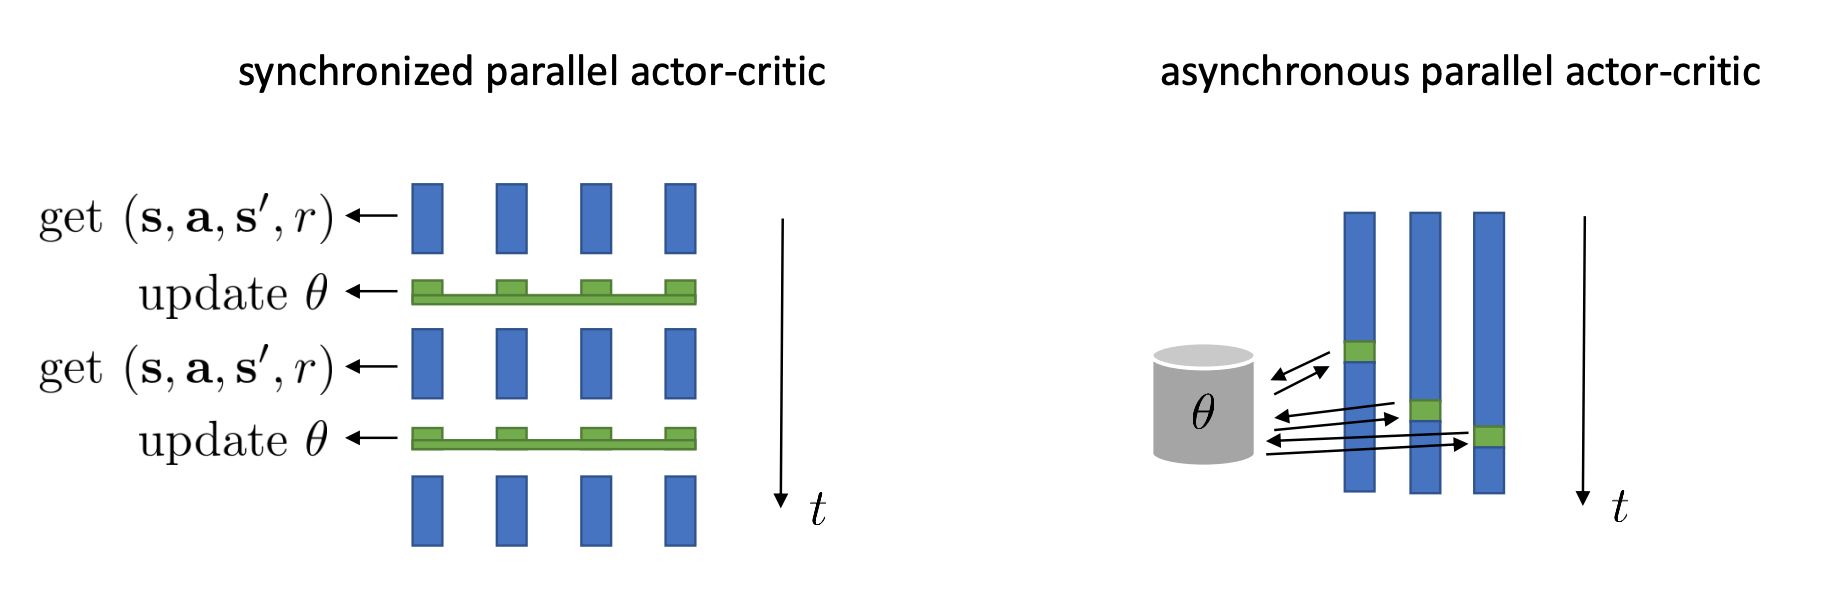
\includegraphics[scale=0.5]{figures/parallelsim.png}
    \caption{Parallel simulations for online actor-critic}
    \label{fig:parallelsim}
\end{figure}

\section{Critics as State-Dependent Baselines}
Now let us further discuss about the connection between a baseline and a critic. Recall in the Monte Carlo version of policy gradient, the gradient is defined as:
$$\nabla_\theta J(\theta) \simeq \frac{1}{N}\sum_{i=1}^N\left(\sum_{t=1}^T\nabla_\theta \log\pi_\theta(a_{i,t}|s_{i,t})\right)\left(\sum_{t'=1}^T r(s_{i,t'},a_{i,t'}) - b\right)$$
and in actor-critic algorithm, we estimate the gradient by estimating the advantage function:
$$\nabla_\theta J(\theta) \simeq \frac{1}{N}\sum_{i=1}^N\left(\sum_{t=1}^T\nabla_\theta \log\pi_\theta(a_{i,t}|s_{i,t})\right)\left(r(s_{i,t},a_{i,t}) + \gamma\hat{V}_\phi^\pi(s_{i,t+1})-\hat{V}_\phi^\pi(s_{i,t})\right)$$

So what are the pros and cons of the two approaches? In policy gradient with baselines, we have shown that there is no bias in our estimation, but there might be high variance due to our single-sample estimation of the cost-to-go function. On the other hand, in the actor-critic algorithm, we have shown that we have lower variance due to the critic, but we end up having a biased estimation because of the possibly bad critic as we are bootstrapping. So can we somehow keep the estimator unbiased while lowering the variance with the critic $\hat{V}^\pi_\phi$?

The solution is obvious and straightforward, we can just use $\hat{V}^\pi_\phi$ in place of $b$:
$$\nabla_\theta J(\theta) \simeq \frac{1}{N}\sum_{i=1}^N\left(\sum_{t=1}^T\nabla_\theta \log\pi_\theta(a_{i,t}|s_{i,t})\right)\left(\sum_{t'=1}^T r(s_{i,t'},a_{i,t'}) - \hat{V}^\pi_\phi(s_{i,t}))\right)$$
In this way, we obtain an unbiased estimator with lower variance. 

\section{Eligibility Traces and n-Step Returns}
In the above comparison of the two methods, we have seen that in the actor-critic advantage function, we have lower variance but higher bias, while in the Monte Carlo policy gradient, the advantage function has lower bias but higher variance. The reason why this tradeoff exists is that as we go further in our trajectory into the future, the variance increases due to the fact that the current single sample approximation is not representative enough for the future. Therefore, the Monte Carlo advantage function is good for getting accurate values in the near term, but not the long term. In contrast, in actor-critic advantage, the bias potentially skews the values in the near term, but the fact that the bias incorporates a lot of states will likely make it a better approximator in the long run. Therefore, it would be better if we could use the actor-critic based advantage for further in the future, and use the Monte Carlo based one for the near term in order to control the bias-variance tradeoff.

As a result, we can cut the trajectory before the variance gets too big. Mathematically, we can estimate the advantage function by combining the two approaches: use the Monte Carlo approach only for the first $n$ steps:
$$\hat{A}^\pi_n(s_t,a_t) = \sum_{t'=t}^{t+n}\gamma^{t'-t}r(s_{t'},a_{t'}) - \hat{V}^\pi_\phi(s_t)+\gamma^n\hat{V}^\pi_\phi(s_{t+n})$$
here we applied an n-step estimator, which sums the reward from now to $n$ steps from now, and $n>1$ often gives us better performance.

Furthermore, if we don't want to choose just one $n$, we can use a weighted combination of different $n$-steps returns, which we can define as the General Advantage Estimation(GAE):
$$ \hat{A}_{GAE}(s_t,a_t) = \sum_{n=1}^\infty w_n \hat{A}^\pi_n(s_t,a_t)$$
To choose the weights, we should prefer cutting earlier, so we can assign the weights accordingly: $w_n\propto \lambda^{n-1}$, where we call $\lambda$ the chance of getting cut.

